\documentclass[11pt,twoside,a4paper]{article}
\usepackage{fancyhdr}
\usepackage[UTF8]{ctex}
\usepackage[centering]{geometry}
\usepackage{graphicx}
\usepackage{setspace}
%\usepackage{listings}
%\usepackage[colorlinks=true,linkcolor=blue,urlcolor=blue,citecolor=black]{hyperref}
%
%\usepackage{algorithm}  
%\usepackage{algorithmicx}  
%\usepackage{algpseudocode}  
%\usepackage{amsmath}  
%\usepackage{graphicx}
\begin{document}
	\begin{figure}[h]
		\centering
		% Requires \usepackage{graphicx}
		
\includegraphics[width=0.8\textwidth]{graph/logo.png}\\
	\end{figure}
\thispagestyle{empty}
\begin{center}
	\doublespacing
	\huge 当代中国医疗的深度思考
	
	\Large 1160300329\ 黄海 
	
	\Large 1160300308\ 干寅雷
	
	\Large 1160300311\ 汤嘉琦
	
	\Large 1160300312\ 靳贺霖
	
	\Large 1160300314\ 朱明彦
\end{center}
	\singlespacing
%	\title{当代中国医疗的深度思考}
%	
%	\author{1160300329\ 黄海\\1160300308\ 干寅雷\\1160300311\ 汤嘉琦\\
%		1160300312\ 靳贺霖\\1160300314\ 朱明彦\\1603003班}
%	\author{Paolo Ienne\\ 
%		Swiss Federal Institute of Technology\\ Microcomputing Laboratory \\ IN-F 
%		Ecublens, 1015 Lausanne, Switzerland\\ Paolo.Ienne@di.epfl.ch\\ 
%		% For a paper whose authors are all at the same institution, 
%		% omit the following lines up until the closing ``}''. 
%		% Additional authors and addresses can be added with ``\and'', 
%		% just like the second author. 
%		\and 
%		Second Author\\ 
%		Institution2\\ 
%		First line of institution2 address\\ Second line of institution2 address\\ 
%		SecondAuthor@institution2.com\\ 
%	} 
	\newpage
	\pagestyle{fancy}
	\thispagestyle{fancy}
	\lhead{当代中国医疗的深度思考}
	\chead{}
	\rhead{Harbin Institute of Technology}
	\lfoot{}
	\cfoot{}
	\rfoot{\thepage}
%	\maketitle
	
	\newpage
	\begin{center}
	\textbf{Abstract}	
	\end{center}
		对于当前的中国医疗,不可否认其中存在问题。在下面的讨论中,我们将对于中国医疗的价格高低,通过对比的方式利用辩证法的原理,进行分析。合理看待中国医疗价格中存在的问题,并探寻问题产生背后的原因。
	\begin{flushleft}
	\textbf{Keyword:中国,\ 医疗问题,\ 医患关系,\ 医疗资源,\ 医疗成本,\ 医疗保险,\ 医疗改革}
	\end{flushleft}

	\newpage
	
	\tableofcontents
	
	\newpage
	
	\section{中国医疗成本}
		\subsection{简述}
		对于中国医疗成本的高低,如果我们仅仅针对中国的情况纵向来看,有失其完整性。基于此,我们使用辩证法的思想,通过对比的方式,将中国与发展中国家代表(印度)以及发达国家代表(美国)进行横向的比较。通过这种方式,进而来说明中国医疗成本在世界中的地位和存在的问题。对于医疗问题中的不同方面,如医务人员薪酬方面,医疗器械方面和药品价格三个方面,使用上面的思路进行分析。
		\subsection{医务人员方面}
		对于中国的医务人员,先说结论:\textbf{在世界的各个国家之中,属于低收入的医务人员群体}。
		
		在这里,我们选取了一个来自中国985院校的医学硕士毕业生(下面简称为“985学生”)作为对比的对象,与中国城镇居民人均收入进行对比。可以发现,985学生的平均收入为$80000$元每年,与其对比的中国的城镇居民的人均收入已经达到了$30000$元每年。
		
		对于个例我们只是作为一种说明,下面借用2016年丁香园医生对于中国医务人员薪酬的调查\cite{ref1}来看,中国的医务人员的平均年薪为$85000$元,对比2016年度全国城镇居民人均可支配收入$33616$元\cite{ref2}来看,已经是其3倍左右,我们可以说医务人员的收入不低,进而我们可以说医疗成本至少不低,因为治病的医生的工资成本很高。但是由于没有很好的中位数数据,可能有不少被平均的情况,我们只能得到以上的结论。
		\begin{figure}[htb]
			\centering
			% Requires \usepackage{graphicx}
			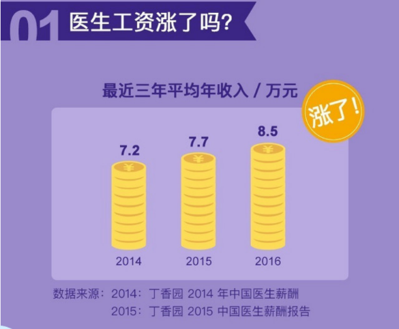
\includegraphics{graph/DingXiangyuan.png}\\
			\caption{丁香园2016年中国医务人员薪酬调查}
		\end{figure}
	
		我们可以看到美国的医生平均收入已经达到了$28$万美元以上\cite{ref3},相比美国人均年收入$42372$美元,已经超出6倍有余,这是中国医生所远远不能与之相比的。
		
		
		再来看印度,由于数据的问题我们不能找到具体的印度医生收入的直接证明,但是相信看过生活大爆炸的同学都会对Raj的父亲的收入有着极深的印象。根据较少数据规模的统计我们可以知道,在印度医生的工资分布比较分散,在印度,一个家庭医生的收入约为16万到126万卢比不等,并且由于印度允许医生在医院之外行医所以工资更加难以计算。我们可以参考的另一个数据是在印度医学院毕业的本科生的薪资一般为1000美元一个月,对比印度的人均年收入1500美元左右,也称得上是高收入人群了。
		
		\begin{figure}[htb]
			\centering
			% Requires \usepackage{graphicx}
			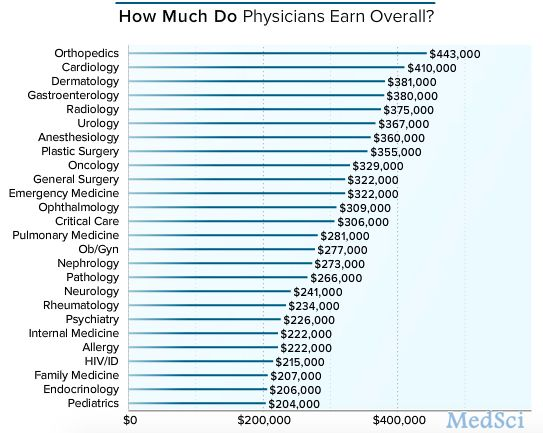
\includegraphics[width=0.8\textwidth]{graph/20160402203312581.png}\\
			\caption{2016年Medscape医生收入调查}
		\end{figure}
		
		另外中国医生除了薪资不高还有这些问题,工作强度大,收入满意度低还有升职加薪困难。这些低收入高压力之间的矛盾让很多医生都不堪重负。
		
		可以说无论是印度还是美国,医生的社会地位和薪资状况在其社会环境中都出于中上地位相比,中国的医生真的可以说是“价廉”了,换句话说医生的薪资很低,中国的医疗成本应该不高。
		
		\subsection{医疗器械方面}
		这个方面我们结合着来看,以心血管支架为例,某种血管支架在我国现行价格为$1.8$万元左右人民币,而产地美国却是$8000$元人民币。中间超过一倍有余的价格都是来自于经销商的层层剥皮。这仅仅是一个方面,同样跟血管支架有着类似情况的医疗器械,小到一个几百美元的血管钳,上到单机价格$2000$万人民币的达芬奇手术机器人,中国无不使用远高于国外价格的来进口,而不能用国产设备代替。
		
		也就是中国无法打破国外的技术壁垒,只能用远低于发达国家国民收入的百姓的辛苦钱去承担与发达国家百姓相同甚至更高的医疗器械费用。
		
		\subsection{药品方面}
		中国是有着几十年不涨价的药物,但是近些年来不断出现的出国去买靶向药的情况屡有发生,这与中国国产没有靶向药不无关系。做一个直接的价格对比“特罗凯(抗癌药)在2016年8月份宣布降价,但仍要$4000$多元一盒。
		
		又如,和特罗凯同属抗癌靶向药的格列卫,国内正版的价格仍要$2$万多元一盒,仿制药物$3000$多元,而印度版格列卫一盒只需$200$多元。”
		
		虽然现在有了医疗报销的体系,在部分发达的地区报销格列卫的比例超过$90\%$,但仍有$2000$多元一盒的高昂价格。这相差十几倍的价格仍然需要中国患者来承担,这些对比我们可以坚定地说中国的医疗成本很高。
		
		\subsection{简要分析}
		结合三个方面辩证来看,我们不能直接说中国的医疗成本很高,因为中国医生收入真的不高;也不能说中国的医疗成本低,因为无论药品或是器械,国内的价格远高于国外。
		
		那么我们只好用事实进行佐证,在现在,即使有着大病保险和医疗保险的极高覆盖,但对于很多的中国居民“一病回到解放前”真的是一种普遍情况,所以我们可以认为中国的医疗成本确实很高,这种高不是来自于平时的头疼脑热所用掉的那些医保以内的药物,而是当真正有着严重疾病发生的时候那种高昂的医疗成本造成的。
		
		\section{中国医改的历程}
		回顾中国医改的历程,我们发现,卫生事业改革发展的过程,就是保障人民健康水平这个根本目标、不断在改革发展中解决新矛盾新问题的过程。
		
		1980年,取消单位医务室,农村合作医疗解体。国务院发文允许个体医生开业行医,民营医疗市场开始兴起,医疗卫生机构开始走向社会化,企业化。1989年,国务院出台意见,强化医疗卫生市场化,实行医院分级管理体制,各级医疗单位内部独立核算、自负盈亏。由于缺乏认证和监管,各地医疗卫生技术水平,收入差距进一步加大。一些医院为了追求利益,开始出现医疗乱象。1998年,中国社会医疗保障体系建设开始。医保改革主要是城市经济体制改革的配套,并稳定剧变中的职工队伍。在很大范围内,将公费医疗制度转为医疗保险制度,由政府全包转向政府主导与市场机制结合。2009年,新一轮医改方案正式出台,提出建立健全医疗保障体系,基本公共卫生服务的均等化,实现‘重治疗“向”重预防“转变的前提。
		
		上述过程可以归结为三个阶段。第一阶段是从1978年至1996年,这一阶段是我国卫生事业解放思想、积极探索的阶段。上世纪70年代末,由于十年动乱的影响,我国医疗卫生资源严重短缺;综合国力和财力较弱,政府发展卫生事业的能力受到极大限制;同时由于平均主义和“大锅饭”盛行,医疗卫生领域服务质量受到诟病。针对医疗服务供不应求的主要矛盾,这一阶段卫生改革发展的重点是大力提高卫生服务能力,增强医疗卫生机构活力,扩大服务供给,缓解供需矛盾。同时要打破“平均主义”和“大锅饭”的分配方式,调动人员积极性,激发活力,提高效率。第二阶段是从1997年至2002年,这一阶段是我国卫生事业明确方向,加快发展的阶段。针对医疗机构的趋利性,1996年底我国召开新中国成立以来的第一次全国卫生工作大会,强调坚持把社会效益放在首位,防止片面追求经济利益而忽视社会效益的倾向;强调优先发展和保证基本卫生服务,体现社会公平;强调合理配置资源等等。第三阶段是从2003年以来至今,随着我国经济社会发展进入新的阶段,我国卫生事业发展坚持以科学发展观为指导,进入了强调公益、改善民生的新阶段。这一阶段大力推进农村卫生建设和城市社区卫生建设,建立新型农村合作医疗制度和社会医疗保障制度。在这一时期,国务院批准实施了公共卫生体系建设的三年规划,基本建成了覆盖城乡、功能比较完善的疾病预防控制和应急医疗救治体系。
		
		在医疗改革的过程中,人民健康处在优先发展的战略地位。坚持以人民健康为中心,以公平可及、群众受益为目标,坚守底线、补齐短板,作出更有效的制度安排,维护基本医疗卫生服务的公益性,使全体人民在共建共享中有更多获得感。卫生服务的公益性,使全体人民在共建共享中有更多获得感。此外,坚持保基本、强基层、建机制。将基本医疗卫生制度作为公共产品向全民提供,推动医疗卫生工作重心下移、医疗卫生资源下沉,提升基层医疗卫生的职业吸引力和服务能力,以问题为导向推动制度创新和攻坚突破。同时,坚持政府主导与发挥市场机制作用相结合。在基本医疗卫生服务领域,坚持政府主导,落实政府责任,适当引入竞争机制。在非基本医疗卫生服务领域,发挥市场活力,加强规范引导,满足多样化、差异化、个性化健康需求。坚持推进供给侧结构性改革,实行政事分开、管办分开、医药分开、营利性和非营利性分开,优化供给侧治理能力和要素配置,提升服务效率和质量。对需求侧进行科学引导,合理划分政府、社会、个人责任,促进社会共治。坚持突出重点、试点示范、循序推进。理清改革内在逻辑,突出重要领域和关键环节,及时总结推广地方经验,发挥重点改革的突破性作用和试点的带动效应。把握好改革的力度和节奏,注重统筹兼顾,积极稳妥推进改革。
		
		在接下来的发展之中,医疗改革将朝着以下方向进行。首先是建立科学合理的分级诊疗制度。坚持居民自愿、基层首诊、政策引导、创新机制,以家庭医生签约服务为重要手段,鼓励各地结合实际推行多种形式的分级诊疗模式,推动形成基层首诊、双向转诊、急慢分治、上下联动的就医新秩序。其次要建立科学有效的现代医院管理制度。深化县级公立医院综合改革,加快推进城市公立医院综合改革。到2020年,基本建立具有中国特色的权责清晰、管理科学、治理完善、运行高效、监督有力的现代医院管理制度,建立维护公益性、调动积极性、保障可持续的运行新机制和科学合理的补偿机制。同时,也需要建立高效运行的全民医疗保障制度。按照保基本、兜底线、可持续的原则,围绕资金来源多元化、保障制度规范化、管理服务社会化三个关键环节,加大改革力度,建立高效运行的全民医疗保障体系。坚持精算平衡,完善筹资机制,以医保支付方式改革为抓手推动全民基本医保制度提质增效。建立起较为完善的基本医保、大病保险、医疗救助、疾病应急救助、商业健康保险和慈善救助衔接互动、相互联通机制。此外,建立规范有序的药品供应保障制度。实施药品生产、流通、使用全流程改革,调整利益驱动机制,破除以药补医,推动各级各类医疗机构全面配备、优先使用基本药物,建设符合国情的国家药物政策体系,理顺药品价格,促进医药产业结构调整和转型升级,保障药品安全有效、价格合理、供应充分。
		
		
		
		\begin{thebibliography}{99}  
			\bibitem{ref1}丁香医生.2016 丁香园医生薪酬报告.
			
			http://www.dxy.cn/bbs/topic/37052139?source=rss
			\bibitem{ref2}国家统计局.2016年度全国居民人均可支配收入.
			
			http://data.stats.gov.cn/easyquery.htm?cn=C01\&zb=A0A01\&sj=2016 
			
			\bibitem{ref3}Medscape.PHYSICIAN COMPENSATION REPORT 2016.
			
			http://www.medsci.cn/article/show\_article.do?id=1d356595875
		\end{thebibliography} 
\end{document}